\documentclass[12pt]{iopart}


%Uncomment next line if AMS fonts required
%\usepackage{iopams}

\begin{document}

\title{SunPy - Python for Solar Physics}

\author{S J Mumford}
\address{Solar Physics \& Space Plasma Research Centre (SP$^{2}$RC), School of 
Mathematics and Statistics, The University of Sheffield, Hicks Building, 
Hounsfield Road, Sheffield, S3 7RH U.K.}

\author{J Bloggs}
\address{Wibble wiblle wiblle}

\ead{sunpy@googlegroups.com}

\begin{abstract}
This paper presents version 0.4 of SunPy a community developed Python package 
for solar physics.

\end{abstract}

\maketitle

\section{Introduction}

Science is driven by the analysis of data. Modern advances in sensor
technology combined with the availability of cheap storage has led to
rapid increases in amount of data available to scientists in almost
every discipline.  Solar physics is no exception to this trend. NASA's
Solar Dynamics Observatory (SDO) satellite, launched in February 2010,
produces over 1 TB of catalogued and stored data per day. Managing and
analysing this mountain of data to enable scientific discovery
requires increasingly sophisticated software tools.  Key qualities
that these tools should have include robustness, ease of use, a
transparent development history, ease of modification, and conformance
to standards.  Software with these qualities provides a strong
foundation which is responsive to the needs of the community as data
volumes grow and science questions evolve.
%schriste - the opening paragraph still needs work
%ji - I had a go.

SunPy aims to provide a free, open-source and openly developed software package 
for the analysis and visualisation of solar data. SunPy makes use of the Python 
programming language and the breadth of high-quality science-focused packages 
written in that language. Python is a general-purpose, 
powerful and easy-to-learn high-level programming language.
According to the 
2014 TIOBE Index\footnote{\url{http://www.tiobe.com/index.php/content/paperinfo/tpci/index.html}},
 Python is one of the top ten most popular programming languages in the world 
and is widely used outside of scientific fields in web development, education 
and `big data' analytics.

The development of a package such as SunPy in Python is made possible by the 
rich ecosystem of scientific packages available in Python. Core packages in this 
ecosystem such as \texttt{NumPy}, \texttt{SciPy} and \texttt{matplotlib} 
provide the basic functionality expected of a scientific programming language: 
\textit{e.g.}, array manipulation, core numerical algorithms and visualisation. 
Built upon these foundations, packages such as \texttt{Astropy}, \texttt{pandas} and 
\texttt{scikit-image} provide more domain-specific functionality.

The design philosophy of SunPy is to provide a clean, simple-to-use, and well 
structured package that provides the \textit{core} tools for solar-physics data analysis. The 
primary focus of SunPy's early development is to provide specialised, linked, 
data types that allow the acquisition, processing and visualisation of all types 
of solar data.

The purpose of this paper is to provide an overview of SunPy's current 
capabilities, an overview of the development model and community aspects of the 
SunPy project, as well as future plans. The latest release of SunPy (0.4)
can be downloaded from
the official website (\url{http://sunpy.org}) or can be installed using 
the Python package index (\mbox{\url{http://pypi.python.org/pypi}}).
%schriste - the mbox prevents latex from breaking the url across different lines.

\section{Core Data Types}\label{sec:DataTypes}

Currently SunPy provides data structures that are specifically designed for the
three primary varieties of solar physics data, namely images, time series, and
spectra. SunPy provides core data types for these using Python classes:
\texttt{Map} (2D spatial data), \texttt{LightCurve} (1D temporal series)
and \texttt{Spectrum}/\texttt{Spectrogram} (1 and 2D spectra). 

The classes provide access to the original data
along with associated metadata and provide appropriate convenience functions to
enable data analysis and visualisation. For each of these classes, the data is
stored in the \texttt{.data} attribute while the metadata is stored 
in the \texttt{.meta}\footnote{Except \texttt{LightCurve} which currently does 
not.} attribute. It is possible to instantiate the data types from various 
different sources: \textit{e.g.}, files, URLs, arrays or time ranges.  In order 
to provide instrument-specific specialisation, all the core SunPy data types 
support subclassing; \textit{e.g.}, \texttt{Map} has an \texttt{AIAMap} 
sub-type. 
Data visualisation is provided by two functions: \texttt{peek()}, for quick 
plotting, and \texttt{plot()}, for plotting with more fine-grained control that 
integrates with \texttt{matplotlib}.


This section will give a brief overview of the \textit{current} functionality 
of each of these data types.

\subsection{Map}\label{ssec:map}
The map data type stores 2D spatial data, such as images of the Sun and 
inner heliosphere. It provides: a wrapper around a \texttt{numpy} data array, 
the images associated spatial coordinates, and other metadata. The \texttt{Map} 
class provides methods for typical operations on 2D data, such as rotation and 
re-sampling, as well as visualisation functionality.
The \texttt{Map} class also provides a convenient interface for loading data 
from a variety of sources, including a FITS file as shown in 
Listing~\ref{code:aia_1}.

The architecture of the map subpackage consists of a template map called
\texttt{GenericMap}, which is a subclass of \texttt{astropy.nddata.NDData}. 
\texttt{NDData} is a generic wrapper around a \texttt{numpy.ndarray} with a 
\texttt{meta} attribute to store metadata.
As \texttt{NDData} is currently still in development, \texttt{GenericMap} does 
not yet make full use of its capabilities, but this inheritance structure 
provides for future integration with \texttt{astropy}. In order to provide 
instrument- or detector-specific integration, \texttt{GenericMap} is designed
to be subclassed. Each subclass of \texttt{GenericMap} can register 
with the \texttt{Map} creation factory, which will then automatically return an instance
of the specific \texttt{GenericMap} subclass dependent upon the data provided. 
SunPy v0.4 has \texttt{GenericMap} specialisations for the following 
instruments: 
\textit{Yohkoh}/SXT, \textit{SOHO}/EIT and LASCO, \textit{RHESSI}, 
\textit{STEREO}/EUVI and COR, \textit{Hinode}/XRT,
\textit{PROBA2}/SWAP, \textit{SDO}/AIA and HMI, 
and \textit{IRIS} SJI frames. 
                        
The \texttt{Map} class stores standard metadata retrieved from the header of 
the image file in the \texttt{meta} attribute and provides convenience 
properties for commonly accessed metadata: e.g., \texttt{instrument}, 
\texttt{wavelength} or \texttt{coordinate\_system}. 
Listing \ref{code:aia_1} demonstrates the quick-look functionality of 
\texttt{Map}.

\begin{listing}[H]
\begin{minted}[bgcolor=bg]{pycon}
>>> import sunpy.map
>>> aiamap = sunpy.map.Map('aia_file.fits')
>>> smap = aiamap.submap([-1200, -200], [-1000, -0])
>>> smap.peek(draw_grid=True)
\end{minted}
\begin{center}
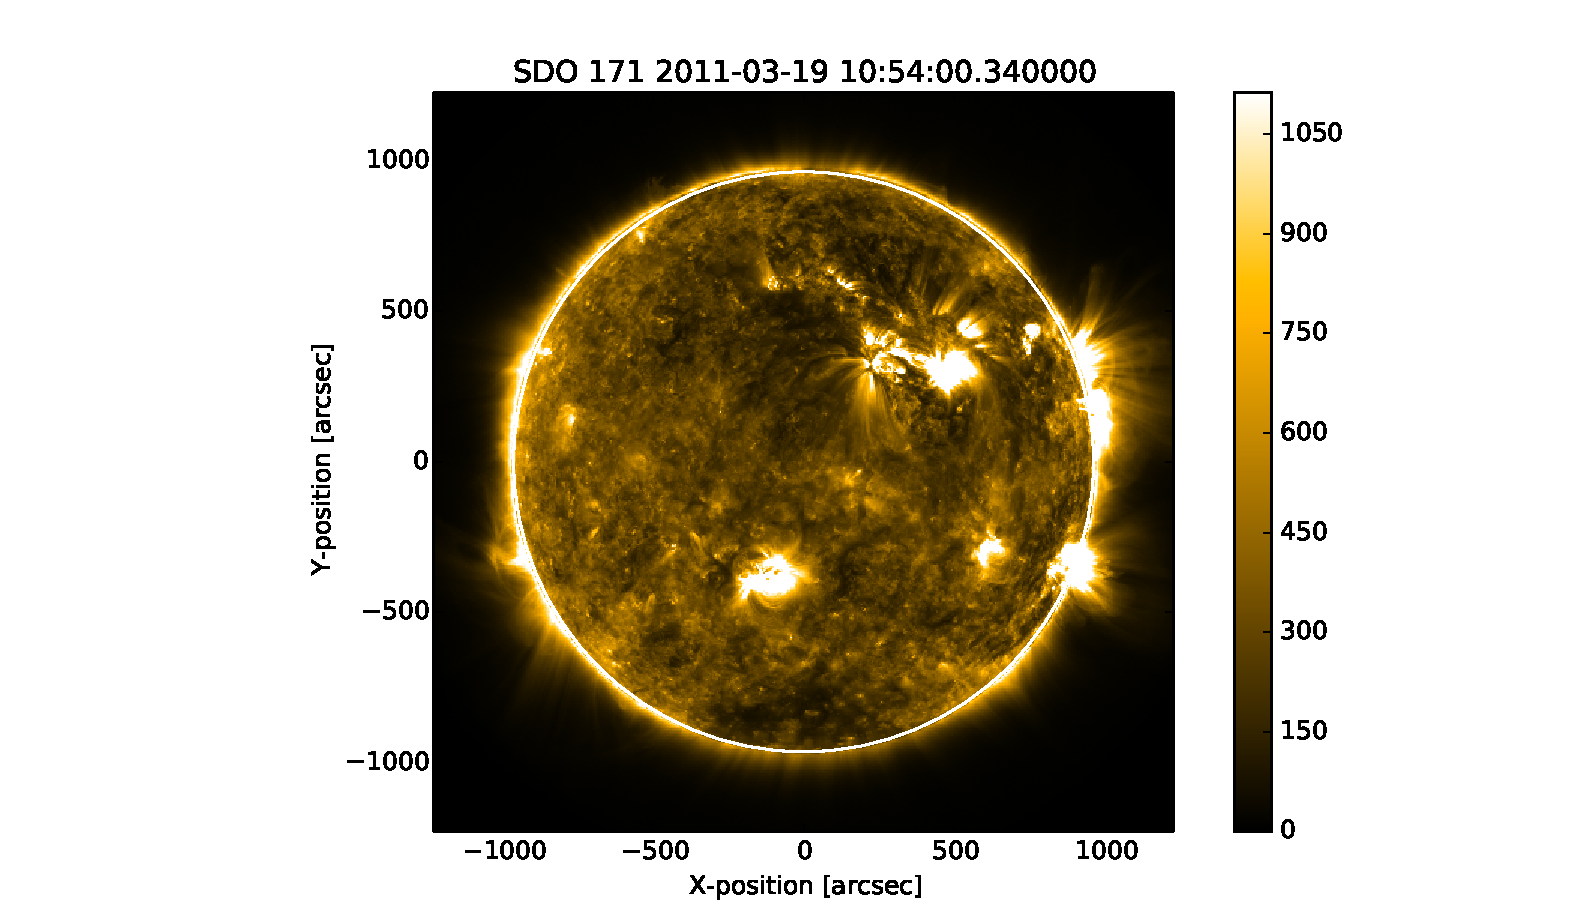
\includegraphics[width=0.8\columnwidth]{aia_map_example}
\end{center}
\caption{Example of the \texttt{AIAMap} specialisation of 
\texttt{GenericMap}. The map is created from an \textit{SDO}/AIA FITS file, a cutout
of the map is created, and then a quick-view plot is created with lines of heliographic longitude and latitude over-plotted.}
\label{code:aia_1}
\end{listing}

In addition to the data-type classes, the \texttt{map} subpackage provides two 
collection classes, \texttt{CompositeMap} and \texttt{MapCube}, for 
temporally and spatially aligned data respectively.
\texttt{CompositeMap} provides methods for overlaying spatially aligned 
data, with support for visualisation of images and contour lines overlaid 
upon each other.
\texttt{MapCube} provides methods for animation of its series of \texttt{Map} 
objects. Listings~\ref{code:compmap_1} and \ref{code:mapcube_1} show how to 
interact with these classes.

\begin{listing}[H]
\begin{minted}[bgcolor=bg]{pycon}
>>> import sunpy.map
>>> import matplotlib.pyplot as plt
>>> compmap = sunpy.map.Map('aia_1600_image.fits', 'RHESSI_image.fits', 
...                         composite=True)
>>> compmap.set_levels(1, range(0,50,5), percent=True)
>>> compmap.set_colors(1, 'Reds_r')
#Plot the result and crop
>>> ax = plt.subplot()
>>> compmap.plot()
>>> ax.axis([200, 600, -600, -200])
>>> plt.show()
\end{minted}
\begin{center}
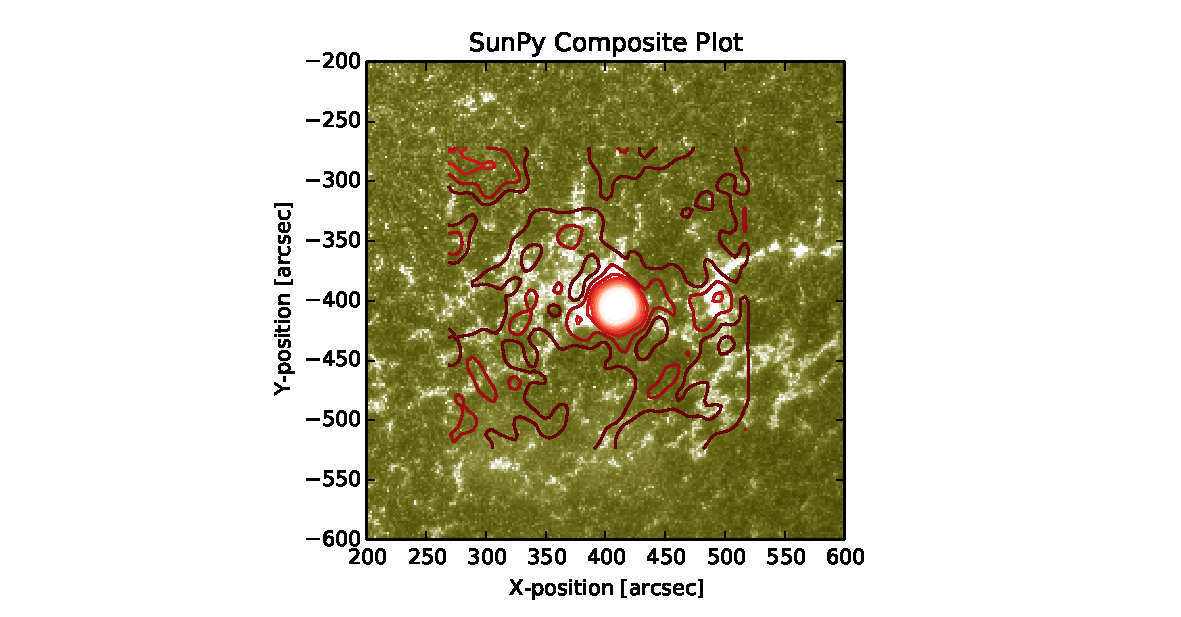
\includegraphics[width=0.8\columnwidth]{comp_map_example}
\end{center}
\caption{Example showing a \texttt{CompositeMap} plot, with RHESSI data composited
with \textit{SDO}/AIA data, and the integration with the \texttt{matplotlib.pyplot} interface.}
\label{code:compmap_1}
\end{listing}

\begin{listing}[H]
\begin{minted}[bgcolor=bg]{pycon}
>>> import sunpy.map
>>> cubemap = sunpy.map.Map('aia_lev1_171a_2014_01*fits', cube=True)
>>> cubemap.peek()
\end{minted}
\begin{center}
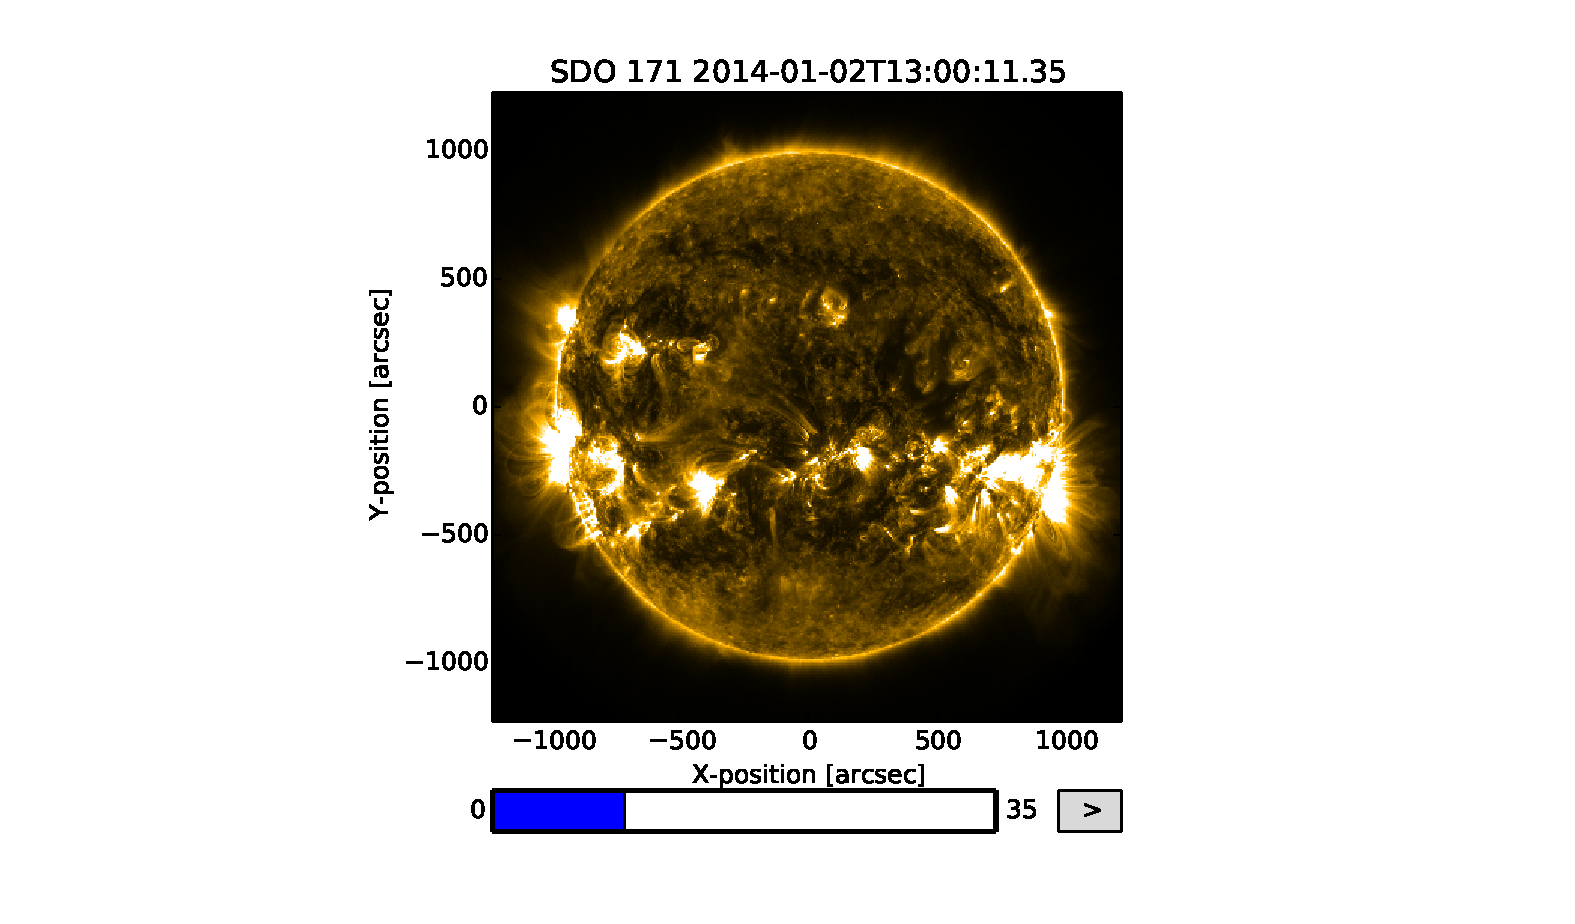
\includegraphics[width=0.8\columnwidth]{aia_cube_controls}
\end{center}
\caption{Example showing creation of a \texttt{MapCube} from a glob file search. The 
resultant plot makes use of \texttt{matplotlib}'s interactive widgets to allow scrolling 
through the \texttt{MapCube}.}
\label{code:mapcube_1}
\end{listing}
\subsection{Lightcurve}\label{ssec:lightcurve}

Time series data and their analyses are a fundamental aspect of solar
physics for which many data sources are available.
SunPy provides a \texttt{LightCurve} class
with a convenient and consistent interface for handling solar time-series
data.  The main engine behind the \texttt{LightCurve} class is
the {\texttt{pandas}} data-analysis library (\url{http://pandas.pydata.org}), and 
\texttt{LightCurve}'s \texttt{data} attribute is a \texttt{pandas.DataFrame} 
object.
The \texttt{pandas} library contains a large amount
of functionality for manipulating and analysing time-series data,
making it an ideal basis for \texttt{LightCurve}.  \texttt{LightCurve}
assumes that the input data are time-ordered list(s) of numbers, and each
list becomes a column in the \texttt{pandas} DataFrame object.

Currently, the \texttt{LightCurve} class is compatible with the
following data sources: the \textit{GOES} X-ray Sensor (XRS), \textit{PROBA2}/LYRA, and
the \textit{SDO} EUV Variability Experiment (EVE; only the level ``OCS'' and
% Do we need to explain what OCS means?
% RJH: I'd argue that everything other than (EVE) can be cut, but I'm not 
% confident enough to make that cut.
% dps: I agree, JI, what do you think?
average CSV files -- see \url{http://lasp.colorado.edu/home/eve/data/}
for more detail).  For each of these instruments, a subclass of the
\texttt{LightCurve} object is initialised
(e.g., \texttt{GOESLightCurve}) which inherits from
\texttt{LightCurve} but allows instrument-specific functionality to be
included.  Future developments will introduce support for additional
instruments and data products, as well as implementing a factory interface 
similar to that of \texttt{Map}.  Since there is no established standard
as to how time-series data should be stored and distributed, each SunPy 
\texttt{LightCurve} object sub-class provides the ability to download its corresponding 
specific data format in its constructor and parse that file type.

A \texttt{LightCurve} object may be created using a number of different methods. 
For example, a \texttt{LightCurve} may be created for a specific instrument given
an input time range. In Listing~\ref{code:goes_lc}, 
the \texttt{LightCurve} constructor searches a remote source for the GOES X-ray 
data specified by the time interval, downloads the required files and 
subsequently creates and plots the object.

%removed the resample part of the example - really we need to fix truncate!
% schriste - i think it would be better to show off some of the powerful pandas methods in this section
% as we are not likely to fix truncate and i think it should be refactored anyway
%ays: moved these comments outside of the listing in case we forget to delete these
\begin{listing}[H]
\begin{minted}[bgcolor=bg]{pycon}
>>> from sunpy import lightcurve
>>> from sunpy.time import TimeRange
>>> goes = lightcurve.GOESLightCurve.create('2011-06-07 06:00',
...                                         '2011-06-07 08:00')
>>> goes.peek()
\end{minted}
\begin{center}
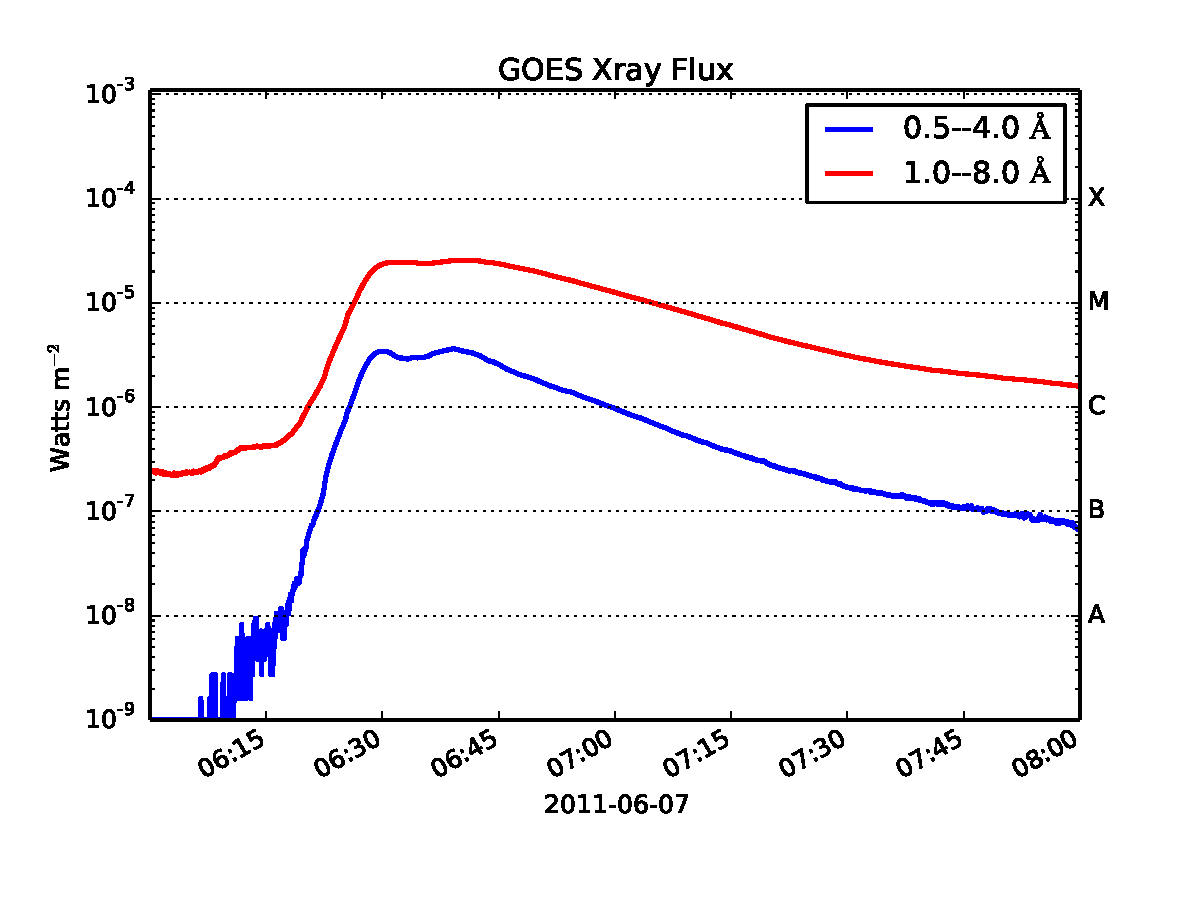
\includegraphics[width=10cm]{goes_lightcurve.pdf}
\end{center}
\caption{Example retrieval of a GOES lightcurve
using a time range, and the output of the 
\texttt{peek()} method.}
\label{code:goes_lc}
\end{listing}
%schriste - note to self, fix this example, add resampled points on top of plot?

Alternatively, if the data file already exists on the local system, the 
\texttt{Lightcurve} object may instead be initialised using that file as input.
Once the \texttt{Lightcurve} has been created, it may be manipulated in 
a variety of ways in order to perform time-series analysis.
%Stuart: Where did the pandas section go?
%ARI - looks like it's up top


\subsection{Spectra}\label{sec:spectra}
%schriste - this section needs major work
%ji - there is no example of a spectrum
%dps - I need to think in one...
%schriste - can't we just take a slice off of the spectram to make a spectrum?

SunPy aims to provide broad support for solar spectroscopy
instruments.  The variety and complexity of these instruments and
their resultant datasets makes this a challenging goal.  The \texttt{spectra} module implements a
\texttt{Spectrum} class for 1D data (intensity as a function of frequency) and a
\texttt{Spectrogram} class for 2D data (intensity as a function of time and
frequency).  Each of these classes use a \texttt{numpy.ndarray} class
as its \texttt{data} attribute.  These two classes were implemented
by funding provided by the Astrophysics Research Group at Trinity
College Dublin, Ireland.

As with other SunPy data types, the \texttt{Spectrogram} class has been
built so that each instrument initialises using a subclass containing the instrument-specific 
functionalities. The common functionality provided by the base \texttt{Spectrogram} class includes
joining different time ranges and frequencies, performing frequency-dependent background subtraction,
and convenient visualization and sampling of the data.
Currently, the \texttt{Spectrogram} class supports radio spectrograms from the 
\href{http://www.e-callisto.org/}{e-Callisto}
solar radio spectrometer network and STEREO/SWAVES spectrograms.

Listing \ref{code:spectra} shows how the \texttt{CallistoSpectrogram}
object retrieves spectrogram data in the time range specified taken at
the observatory of interest.  When the data is requested using the
\texttt{from\_range()} function, the object merges all the downloaded
files into a single spectrogram, across time and frequency.
In the example shown, data is provided in two frequency ranges, 
20--90\,MHz and 55--355\,MHz.  Since the data is not evenly spaced in
the frequency range, the \texttt{Spectrogram} object linearises the
frequency axis for a better analysis.  The example also demonstrates
the implemented background subtraction method.
% RJH: Which subtraction method?  If the specifics are irrelevant, cut it.
%ji to DPS - what is the linearisation that is happening here?

\begin{listing}[H]
\begin{minted}[bgcolor=bg]{pycon}
>>> from sunpy.spectra.sources.callisto import CallistoSpectrogram
>>> tstart, tend = "2011-06-07T06:00:00", "2011-06-07T07:45:00"
>>> callisto = CallistoSpectrogram.from_range("BIR", tstart, tend)
>>> callisto_nobg = callisto.subtract_bg()
>>> callisto_nobg.peek(vmin = 0)
\end{minted}
\begin{center}
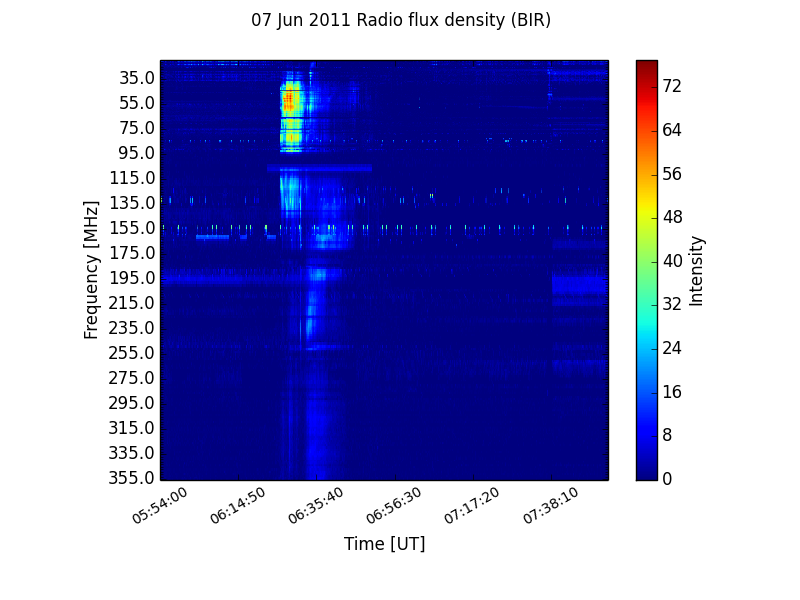
\includegraphics[width=0.8\columnwidth]{callisto_nobg}
\end{center}
\caption{Example of how \texttt{CallistoSpectrogram} retrieves the
  data for the requested time range and observatory, merges it and
  removes the background signal.  The data requested -- `BIR' -- is
  the code name of the \href{http://www.rosseobservatory.ie}{Rosse Observatory}
  at Birr Castle in Ireland.}
\label{code:spectra}
\end{listing}

% Download Callisto
% Merge multiple time-ranges / frequencies (just work from downlad!)
% Merge callisto with swaves



\subsection{Visualisation}
\label{subsec:Viz}
As has been demonstrated in this section, the core SunPy datatypes 
include visualisation code that is tailored to that data type. 
These visualisation methods all currently utilise the \texttt{matplotlib} 
package, and are designed in such a way that they integrate well with 
the \texttt{pyplot} functional interface of \texttt{matplotlib}.

This design philosophy makes the behaviour of SunPy's visualisation 
routines intuitive to those who already understand the \texttt{matplotlib}
interface, as well as allowing the use of the standard 
\texttt{matplotlib} commands to manipulate the plot parameters, such as the 
title.

\section{Solar Data Search and Retrieval}\label{sec:retrieval}

Several well-developed resources currently exist within heliophysics which provide event databases, 
remote access and data retrieval for a large number of data sources. As a community-based project, 
SunPy provides support for these resources via the \texttt{sunpy.net} package. 
In the following subsections, we describe a number of these resources and 
introduce current methods for accessing them within SunPy.

\subsection{VSO}\label{ssec:vso}

The Virtual Solar Observatory (VSO, \url{http://virtualsolar.org}) provides a 
single, standard query interface to solar data from many different archives 
around the world \citep{hill2009}.
Data products can be requested for specific instruments or missions and
can also be requested based on physical parameters of the data product such
as the wavelength range.
In addition to the VSO's primary web-based interface, a SOAP (Simple Object 
Access Protocol) service is also available.
SunPy's \texttt{vso} module provides access to the VSO via this SOAP service using the
\texttt{suds} package.

Listing~\ref{code:vso_query_simple} shows an example of how to query and download data
from the VSO using the \texttt{vso} module.
Queries are constructed using one or more attribute objects. Each
attribute object is a constraint on a parameter of the data set, such as the
time of the observation, instrument, or wavelength.
Listing~\ref{code:vso_query_simple} also shows how to download the data using
the constructed query. The path to which the data files will be downloaded is defined using custom tokens
which reference the file metadata (e.g., instrument, detector, filename). This provides
users the ability to organize their data into subdirectories on download.

Listing~\ref{code:vso_query_advanced} shows an example of how to make an advanced
query by combining attribute objects.
Two attribute objects can be combined with a logical \texttt{or} operation
using the \texttt{|} (pipe) operator.
All attribute objects provided to the query as arguments are combined with a 
logical \texttt{and} operation.

\begin{listing}[H]
\pythoncode{pycode_vso1.txt}
\caption{Example of querying a single instrument over a time range and downloading the data}
\label{code:vso_query_simple}
\end{listing}

\begin{listing}[H]
\pythoncode{pycode_vso2.txt}
\caption{Example of an advanced VSO query using attribute objects,
combining both data from a detector and any data that falls within two wavelength ranges,
continuing from Listing~\ref{code:vso_query_simple}.}
\label{code:vso_query_advanced}
\end{listing}

\subsection{HEK}\label{ssec:hek}

The Sun is an active star and exhibits a wide range of transient phenomena 
(e.g., flares and radio bursts) on many different time-scales, length-scales and 
wavelengths. Observations and metadata concerning these phenomena are collected 
in the Heliophysics Event Knowledgebase (HEK) \citep{hek2012}.  Entries are generated both by 
automated algorithms and human observers.  Some of the information in the HEK 
reproduces feature and event data from elsewhere (for example, the GOES flare catalogue),
and some is generated by the Solar Dynamics Observatory Feature Finding Team 
\citep{martens2012}.  The advantage of the HEK is it 
provides an homogeneous and well-described interface to a large amount of 
feature and event information of interest to the solar physics community.


SunPy accesses this information through the \texttt{hek} module, which was
developed with support from ESA's SOCIS 2011.  The \texttt{hek} module makes 
use of the 
\href{http://vso.stanford.edu/hekwiki/ApplicationProgrammingInterface?action=print}{HEK
 API}.
The current list of events maintained by the HEK and their properties can be 
found at \url{http://www.lmsal.com/hek/VOEvent_Spec.html}.

Simple HEK queries consist of start time, an end time, and an event type 
(Listing \ref{code:hek:simple}). Event types are specified as upper case, 
two letter strings, and are 
identical to the two letter abbreviations found at the HEK website, 
\url{http://www.lmsal.com/hek/VOEvent_Spec.html}.

\begin{listing}[H]
\begin{minted}[bgcolor=bg]{pycon}
>>> from sunpy.net import hek
>>> client = hek.HEKClient()
>>> tstart, tend = '2011/08/09 00:00:00', '2011/08/10 00:00:00'
>>> result = client.query(hek.attrs.Time(tstart,tend), 
...                       hek.attrs.EventType('FL')) # 'FL' indicates flare
>>> len(result)
52
\end{minted}
\caption{Example usage of the \texttt{hek} module showing a simple HEK search for solar flares
which occurred on August 9th, 2011.}
\label{code:hek:simple}
\end{listing}

The module \texttt{hek.attrs} contains attributes of the HEK that can be used to
construct HEK queries.  For example, a flare is an attribute of the HEK, and so 
instead of specifying \texttt{hek.attrs.EventType('FL')} as in Listing 
\ref{code:hek:simple}, this can also be expressed as \texttt{hek.attrs.FL}. 

HEK attributes differ from VSO attributes (Section \ref{ssec:vso}) in that many 
of them are wrappers that conveniently expose comparisons by overloading Python 
operators. This allows filtering of the HEK entries by the properties of the 
event. As was mentioned above, the HEK stores feature/event metadata obtained 
in different ways, known generally as {\it feature recognition methods} (FRMs). 
Example in Listing~\ref{code:hek:frm} filters the results of the previous 
result to return only those events that have the FRM 'SSW Latest Events'.  Multiple comparisons can be made by including more comma-separated
conditions on the attributes in the call to the HEK query method.
\begin{listing}[H]
\begin{minted}[bgcolor=bg]{pycon}
>>> result = client.query(hek.attrs.Time(tstart,tend), 
...                       hek.attrs.EventType('FL'),
...                       hek.attrs.FRM.Name == 'SSW Latest Events')
>>> len(result)
9
\end{minted}
\caption{An HEK query that returns only those flares that were
  detected by the 'SSW Latest Events' feature recognition method.}
\label{code:hek:frm}
\end{listing}

HEK comparisons can be combined using Python’s logical operators e.g. \texttt{and}
and \texttt{or}. This makes complex queries easy to create: Listing \ref{code:hek:or} 
returns flares west of 50 arcseconds or those that have a peak flux above 
1000.0 (the units of the flux are FRM dependent and are described at the HEK 
website).
\begin{listing}[H]
\begin{minted}[bgcolor=bg]{python}
>>> result = client.query(hek.attrs.Time(tstart,tend), 
...                       hek.attrs.EventType('FL'),
...                       (hek.attrs.Event.Coord1 > 50) 
...                       or (hek.attrs.FL.PeakFlux > 1000.0))
\end{minted}
\caption{HEK query using the 'or' operator.}
\label{code:hek:or}
\end{listing}
All FRMs report the required feature attributes (as described at 
\url{http://www.lmsal.com/hek/VOEvent_Spec.html}), but the optional attributes 
are FRM dependent.  If a FRM does not have one of the optional attribute, 
\texttt{None} is returned by the \texttt{hek} module. 

The ability to use comparison and logical operators on HEK attributes allows 
the construction of queries of almost arbitrary complexity. 
The results of a HEK query can be used to download the 
corresponding data from the VSO using SunPy's \texttt{H2VClient}.
%schriste - this is a weird way to end this section, either show how it is done or 
% do not mention it, i think.
%dps - I agree.
%Stuart: Will do on my next pass

\subsection{HELIO}\label{ssec:helio}

The HELiophysics Integrated Observatory (\href{http://helio-vo.eu}{HELIO}) has 
put together a list of web services which allows scientists to query and 
discover data throughout the heliosphere, from solar, and magnetospheric to planetary and 
inter-planetary data \citep{dps2012}.
HELIO has been built with a Service-Oriented Architecture, 
\textit{i.e.} its capabilities are split into a number of tasks that are 
implemented as separate services. 
\href{http://helio-vo.eu}{HELIO} comprises nine different public services, 
which allows scientists to search different catalogues of registered events, 
solar features, data from instruments in the heliosphere and other information 
like planets or spacecraft position in time. 
Additionally, \href{http://helio-vo.eu}{HELIO} provides a service that uses a 
propagation model to link the data in different points of the solar system by 
its original nature (\textit{e.g.}, Earth auroras are a signature of magnetic 
field disturbances produced few days before on the Sun).
In addition to the primary, web-based interface to 
\href{http://helio-vo.eu}{HELIO}, the services can be separately accessed.

SunPy's \texttt{hec} module provides an interface to the
\textit{HELIO Event Catalogue} (HEC) service (not to be confused with the HEK, discussed in Section \ref{ssec:hek}), and this module was developed as
part of a Google Summer of Code (GSOC) project in 2013.
The HEC service currently provides access to 84 catalogues from different
sources.
As with all of the HELIO services, the HEC service provides results in VOTable 
data format (defined by IVOA \cite{ochsenbein_ivoa_2011}), and the \texttt{hec}
module parses this output using the \texttt{astropy.io.votable} package.
This format has the advantage of containing metadata with information like
data provenance and the performed query.

Listing~\ref{code:helio} shows an example of how to obtain information
from different catalogues of coronal mass ejections (CMEs).

\begin{listing}[h]
\begin{minted}[bgcolor=bg]{pycon}
>>> from sunpy.net.helio import hec
>>> hc = hec.Client()
>>> tstart, tend = '2011-06-07T06:00:00', '2011-06-07T12:00:00'
>>> event_type = 'cme'

# From all the catalogues these which name contain our event of interest
>>> catalogues = hc.get_table_names()
>>> catalogues_event = [l[0] for l in catalogues 
...                     if event_type in l[0] and 'list' not in l[0]]

# Query all the catalogues that comes from cactus
>>> results = [hc.time_query(tstart, tend, event) 
...            for event in catalogues_event if 'cactus' in event]
>>> for cat in results:
...     print "{cat} has {nres} results".format(cat = cat.ID, \
...                                             nres = len(cat.array))
__helio_hec-cactus_stereoa_cme has 4 results
__helio_hec-cactus_stereob_cme has 3 results
__helio_hec-cactus_soho_cme has 7 results
\end{minted}
\caption{Example of querying the HEC service to multiple cme
catalogues, in this case the ones detected by \href{http://sidc.oma.be/cactus/}{CACTus}.}
\label{code:helio}
\end{listing}

Additional HELIO services will be supported in the future by SunPy.

\subsection{Helioviewer}\label{ssec:hv}

SunPy provides the ability to download images from Helioviewer Project
servers.  The aim of the Helioviewer Project is to enable the
exploration of solar and heliospheric data from multiple data sources
(such as instrumentation and feature/event catalogs) via easy-to-use
visual interfaces.  The primary data provided by the Helioviewer
Project are images in the JPEG2000 format (for further details on the
Helioviewer Project see \cite{}\footnote{SunPy is used in Helioviewer
  production servers to manage the download and ingestion of JPEG2000
  files from remote servers.}.)  The JPEG2000 files are typically
highly compressed compared to the source FITS files they are generated
from, and so can be a used as a shortcut to visualize large amounts of
data from multiple sources.

The Helioviewer Project categorizes image data based on the physical
construction of the source instrument, using the following hierarchy:
observatory $\rightarrow$ instrument $\rightarrow$ detector
$\rightarrow$ measurement, where '$\rightarrow$' means 'provides
(possibly multiple)'.  The full list of image data sources available
can be found through the code snippet, Example
\ref{code:hv:datasources}.

\begin{listing}
\begin{minted}{python}
from sunpy.net.helioviewer import HelioviewerClient

hv = HelioviewerClient()
datasources = hv.get_data_sources()

# print a list of datasources and their associated ids
for observatory, instruments in datasources.items():
    for inst, detectors in instruments.items():
        for det, measurements in detectors.items():
            for meas, params in measurements.items():
                print("%s %s: %d" % (observatory, params['nickname'], params['sourceId']))
\caption{Initializing the Helioviewer client and listing the full
  range of image data available.}
\label{code:hv:datasources}
\end{listing}

Each Helioviewer Project JPEG2000 file contains metadata which are
based (in part) on the original FITS header information, and carry
sufficient information to permit overlay with other Helioviewer
JPEG2000 files. Images can be accessed either as PNGs (Section
\ref{sssec:hv:png} or as JPEG2000 files (Section \ref{sssec:hv:jp}).

\subsubsection{Download a PNG file}\label{sssec:hv:png}

Example \ref{code:hv:downloadlatestpng} demonstrates how to download a
PNG image of the latest AIA 304\AA\ image available on
Helioviewer.org.

\begin{listing}
\begin{minted}{python}
hv.download_png('2099/01/01', 4.8, "[SDO,AIA,AIA,304,1,100]", x0=0, y0=0, width=512, height=512)
\end{minted}
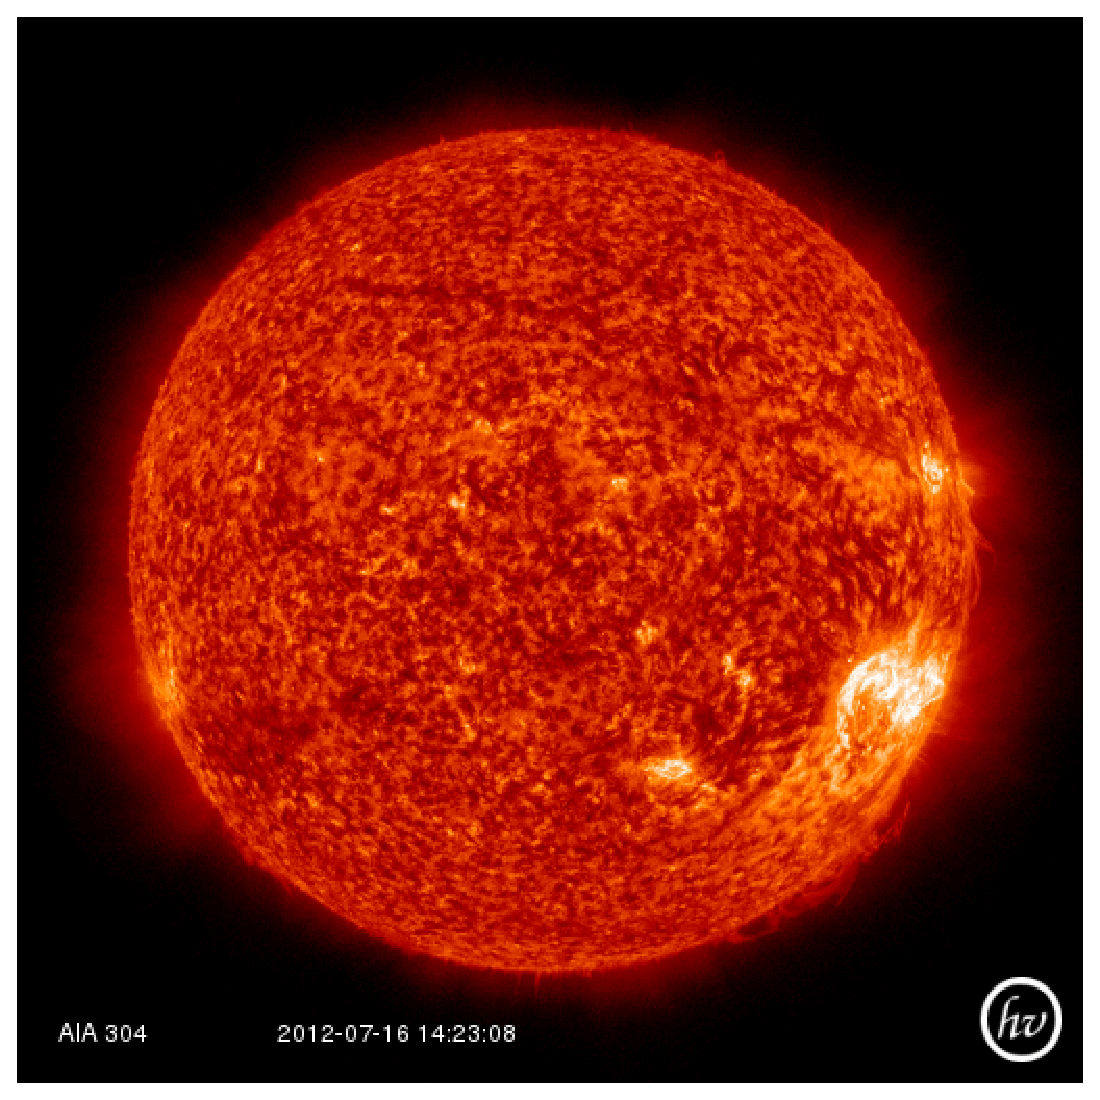
\includegraphics[width=0.8\columnwidth]{helioviewer_latest_aia_304.eps}
\caption{Acquisition of a PNG file showing the latest AIA 304\AA\ image available at
  www.helioviewer.org.}
\label{code:hv:downloadlatestpng}
\end{listing}

The first argument is the requested time of the image.  Helioviewer
selects images closest to the requested time.  In this case, the
requested time is in the future and so Helioviewer will find the most
recent available image.  The second argument refers to the image
resolution in arcseconds per pixel (larger values mean lower
resolution).  The third argument is a string detailing the requested
observatory $\rightarrow$ instrument $\rightarrow$ detector
$\rightarrow$ measurement combination.  The final two numbers in this
string are the visibility and the opacity of the this image layer (1/0
is visible/invisible with opacity in the range $0\rightarrow100$, with
$100$ meaning fully opaque).  The quantities $x0$ and $y0$ are the $x$
and $y$ center points about which to center the image (measured in
helio-projective cartesian co-ordinates) and the \texttt{width} and
\texttt{height} are the pixel values for the image dimensions.

It should be noted that the filename of the returned file has the date
and time of the requested time, which is not the time of the
observation shown in the PNG image.  This is because of the
Helioviewer API.  The API request finds images closest to the
requested time. But since the user may ask for images from multiple
sources, and each of them may have a different observation time, it is
unclear which time is the most appropriate to associate with the
resultant image.  The Helioviewer API does not select between any of
the image observation times, but instead returns an image filename
based on the request time, resulting in predictable filenames.

The Helioviewer API allows composition and overlay of images from
multiple sources, based on the positioning metadata in the source FITS
file.  SunPy accesses this overlay/composition capability through the
\texttt{download_png} method of the Helioviewer client.  Example
\ref{code:hv:overlaid} gives an example of the composition of three
separate images in to a single image.

\begin{listing}
\begin{minted}{python}
hv.download_png('2099/01/01', 6, "[SDO,AIA,AIA,304,1,100],[SDO,AIA,AIA,193,1,50],[SOHO,LASCO,C2,white-light,1,100]", x0=0, y0=0, width=768, height=768)
\end{minted}
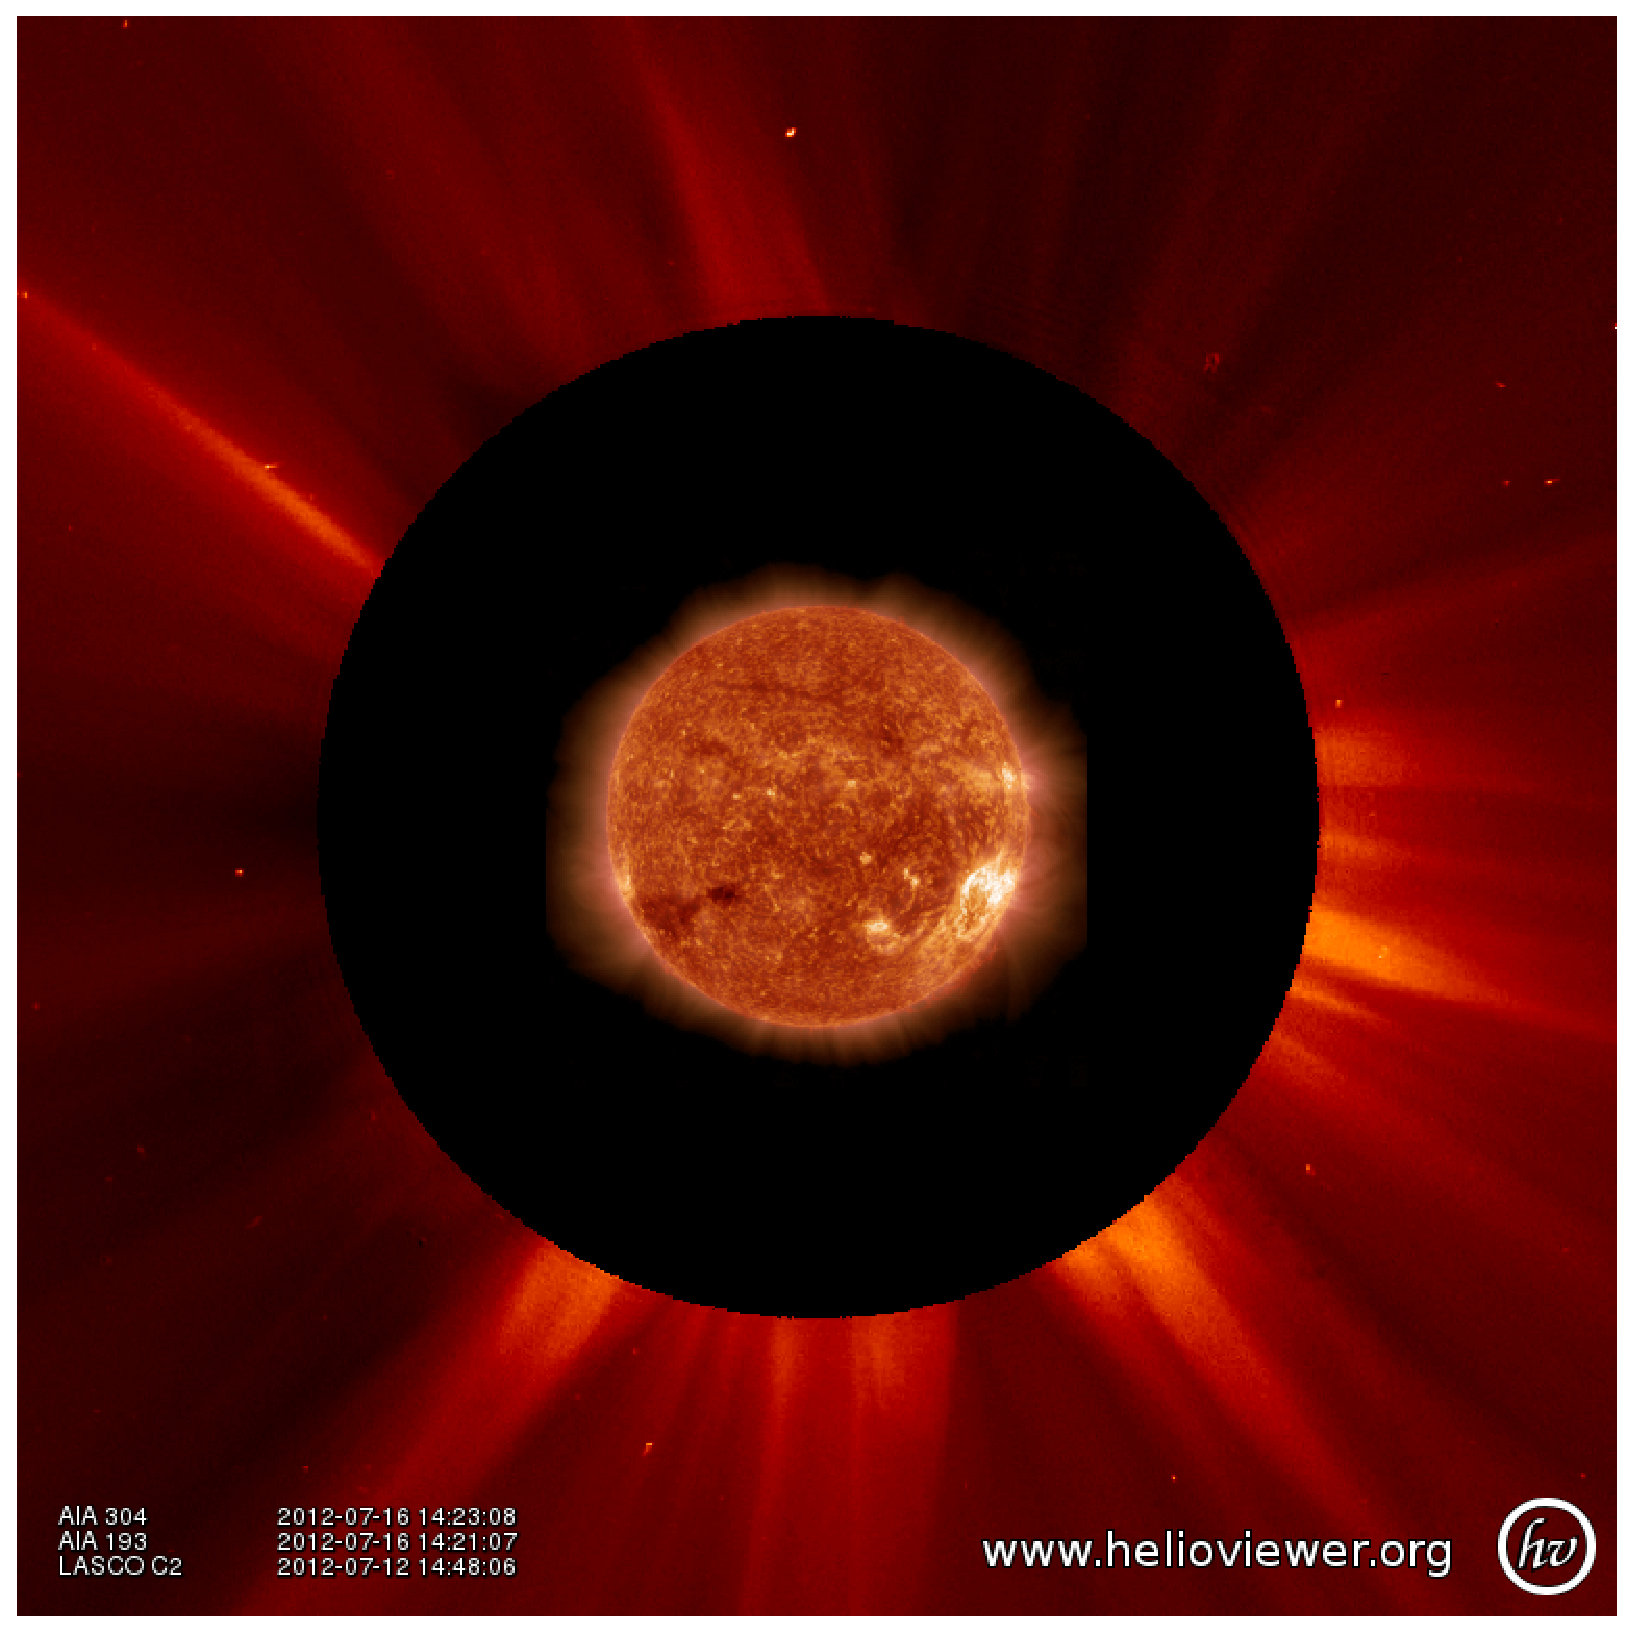
\includegraphics[width=0.8\columnwidth]{helioviewer_overlay_example.eps}
\caption{Acquisition of a PNG image composed from data from three
  separate sources.}
\label{code:hv:overlaid}
\end{listing}

The principle difference between this code snippet and Example
\ref{code:hv:downloadlatestpng} is in the layer string (the third
argument).  The layer string has three separate comma separated
entries detailing the data source, its visibility and its opacity.
This functionality makes it simple for SunPy users to generate complex
images from multiple, correctly overlaid, image data sources.


\subsubsection{Download a JPEG2000 file}\label{sssec:hv:jp}

As noted above, Helioviewer JPEG2000 files contain metadata that allow
positioning of the image data.  There is sufficient metadata in each
file to permit the creation of a SunPy map object (see Section
\ref{ssec:maps}) from a Helioviewer JPEG2000 file.  This allows image
data to be manipulated in the same way as any other map object.

Reading JPEG2000 file into a SunPy session requires installing two
other pieces of software. The first, \texttt{OpenJPEG}, is an open
source library for reading and writing JPEG2000 files
(http://www.openjpeg.org).  The other package required is
\texttt{glymur}, (https://github.com/quintusdias/glymur), an interface
between Python and the OpenJPEG libraries (note that these packages
are {\it not} required to use the functionality described in Section
\ref{sssec:hv:png}).

Listing \ref{code:downloadjp2} demonstrates the querying, downloading,
reading and conversion of a Helioviewer JPEG2000 file into a SunPy Map
object.  This functionality allows users to visualize and manipulate
Helioviewer-supplied image data in an identical fashion to a SunPy map
object generated from FITS data (see Section \ref{sec:maps}).

\begin{listing}
\begin{minted}{python}
filepath = hv.download_jp2('2012/07/05 00:30:00', observatory='SDO', instrument='HMI', detector='HMI', measurement='continuum')
from sunpy.map import Map
hmi = Map(filepath)
hmi.submap([200,550],[-400,-200]).peek()
\end{minted}
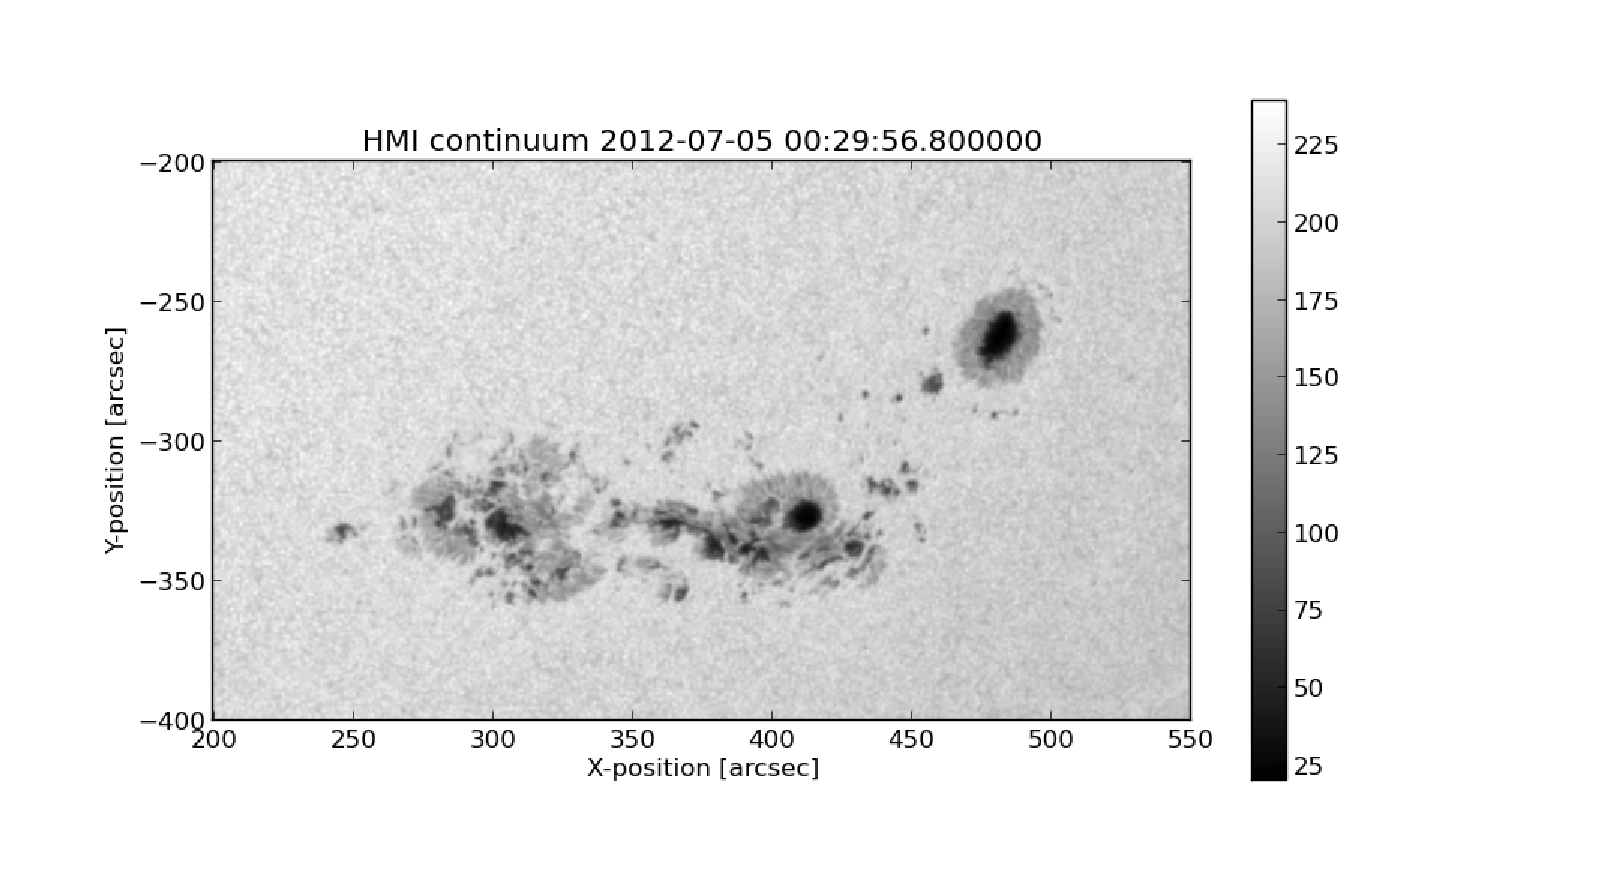
\includegraphics[width=0.8\columnwidth]{helioviewer_hmi_continuum_jp2_to_map.eps}
\caption{Acquisition and display of a Helioviewer JPEG2000 file as a
  SunPy map object.}
\label{code:downloadjp2}
\end{listing}



%
% Helioviewer article citation
%
%@article{Muller:2009:JVL:2220073.2220164,
% author = {Muller, D. and Fleck, B. and Dimitoglou, G. and Caplins, B. W. and Amadigwe, D. E. and Ortiz, J. P.G. and Wamsler, B. and Alexanderian, A. and Hughitt, V. K. and Ireland, J.},
% title = {JHelioviewer: Visualizing Large Sets of Solar Images Using JPEG 2000},
% journal = {Computing in Science and Engg.},
% issue_date = {September 2009},
% volume = {11},
% number = {5},
% month = sep,
% year = {2009},
% issn = {1521-9615},
% pages = {38--47},
% numpages = {10},
% url = {http://dx.doi.org/10.1109/MCSE.2009.142},
% doi = {10.1109/MCSE.2009.142},
% acmid = {2220164},
% publisher = {IEEE Educational Activities Department},
% address = {Piscataway, NJ, USA},
% keywords = {data visualization},
%} 
\subsection{The File Database}\label{ssec:db}

Easy access to large quantities of solar data frequently leads to data files accumulating
in local storage such as laptops and desktop computers. Keeping data organised and available
is typically a cumbersome task for the average user. The file database is a sub-package of 
SunPy which is meant to solve this problem by providing a unified database to store and 
manage information about local data files. The database package was developed with support from 
the Google Summer of Code (GSoC) program 2013.

The database sub-package makes use of a database supported by
\href{http://www.sqlalchemy.org}{SQLAlchemy}. This library was chosen
since it supports many SQL dialects. 
If SQLite is selected, the database is stored as a single file which is
created automatically. A server-based database, on the other hand, could be used
by a collaborators who work together on the
same data from different computers: a central database server stores all data and the clients connect to
it to read or write data.

The database can store and manage all data that can be read via SunPy's 
\texttt{io} subpackage, and direct integration with the \textsc{VSO} 
subpackage is supported.
It is also possible to manually add file or directory entries. The package also provides
a unified data search via the \texttt{fetch()} method, which includes both local files
and files on the \textsc{VSO}. This reduces the likelihood of downloading the same file 
multiple times. When a file is added to the database, the file is scanned and a file hash is produced. 
The current date is associated with the entry along with metadata summaries such 
as instrument, date of observation, field of view, etc. 
The database also provides the ability to associate custom meta-data to 
each database entry such as keywords, comments, and favouring, as well as 
querying the full metadata (i.e., FITS header) of each entry.

The \texttt{Database} class connects to a database and allows the user to 
perform operations on it. Listing~\ref{code:database} shows how to connect
to an in-memory database and download data from the \textsc{VSO}. These entries are
automatically added to the database. The function \texttt{len()} is used to get the number of
records. The function \texttt{display\_entries()} displays an iterable of 
database entries in a nicely-formatted \textsc{ASCII} table. The headlines 
correspond to the attributes of the respective database entries.

A very special feature of the database package is the support of \texttt{undo}
and \texttt{redo} operations. This is particularly convenient in
interactive sessions to easily revert accidental operations. 
This feature will also be desirable when creating a GUI frontend for this package.

\begin{listing}[H]
\begin{minted}[bgcolor=bg]{pycon}
>>> from sunpy.net import vso
>>> from sunpy.database import Database
>>> database = Database('sqlite:///')
>>> database.download(
...     vso.attrs.Time('2012-08-05', '2012-08-05 00:00:05'),
...     vso.attrs.Instrument('AIA'))
>>> len(database)
2
>>> from sunpy.database.tables import display_entries
>>> print display_entries(
...     database,
...     ['id', 'observation_time_start', 'wavemin', 'wavemax'])
id observation_time_start wavemin wavemax
-- ---------------------- ------- -------
1  2012-08-05 00:00:01    9.4     9.4    
2  2012-08-05 00:00:02    33.5    33.5   
\end{minted}
\caption{Example usage of the database sub-package.}
\label{code:database}
\end{listing}



\section{Additional Functionality}\label{sec:util}
SunPy is meant to provide a consistent environment for solar data analysis. In 
order to achieve this goal SunPy provides a number of additional functions and packages which 
are used by the other SunPy modules and are made available to the user. This section 
briefly describes some of these functions.
	
\subsection{World Coordinate System (WCS) Coordinates}\label{ssec:util:wcs}
Coordinate transformations are frequently a necessary task within the solar 
data analysis workflow. An often used transformation is from 
observer coordinates (e.g., sky coordinates) to a coordinate system that is 
mapped onto the solar surface (e.g., latitude and longitude). This 
transformation is necessary to compare the true physical distance between 
different solar features. This type of transformation is not unique
to solar observations, but is not often considered by astronomical packages
such as the Astropy 
\texttt{coordinates} package. The \texttt{wcs} package in SunPy implements the World Coordinate 
System (WCS) for solar coordinates as described by \cite{thompson2006}. The 
transformations currently implemented are some of the most commonly used in solar data analysis, namely converting from Helioprojective-Cartesian 
(HPC) to Heliographic (HG) coordinates. HPC describes the positions on 
the Sun as angles measured from the center of the solar disk (usually in 
arcseconds) using Cartesian coordinates (X, Y). This is the coordinate system 
most often defined in solar imaging data (see for example, images from 
\textit{SDO}/AIA, \textit{SOHO}/EIT, and \textit{TRACE}). 
HG coordinates express positions on the Sun using longitude and latitude on 
the solar sphere. There are two standards for this coordinate system:
Stonyhurst-Heliographic, where the origin is at the intersection of the solar 
equator and the central meridian as seen from Earth, and 
Carrington-Heliographic, which is fixed to the Sun and does not depend on Earth. The 
implementation of these transformations pass through a common coordinate system 
called Heliocentric-Cartesian (HCC), where positions are expressed in true 
(de-projected) physical distances instead of angles on the celestial sphere.
These transformations require some knowledge of the location of the observer, 
which is usually provided by the image header. In the cases where it is 
not provided, the observer is assumed to be at Earth. Listing \ref{code:wcs_code} shows 
some examples of coordinate transforms carried out in SunPy using the 
\texttt{wcs} utilities. 

\begin{listing}[H]
\pythoncode{pycode_util1.txt}
\caption{Using the \texttt{wcs} subpackage.}
\label{code:wcs_code}
\end{listing}

\subsection{Solar Constants and units}\label{ssec:util:sun}
Physical quantities (i.e. a number associated with a unit) are an important part
of scientific data analysis. SunPy makes use of the \texttt{Quantity} object provided by 
Astropy \texttt{units} package. This object maintains the relationship between 
a number and its unit and makes it easy to convert between units. 
As these objects inherit from 
NumPy's \texttt{ndarray}, they work well with standard representations of numbers. Using proper
quantities inside of the code base also makes it easier to catch errors in calculations.
SunPy is currently working on integrating quantities throughout the code base.
In order to encourage the use of units and to enable consistency SunPy provides
the \texttt{sun} subpackage which includes solar-specific data such as ephemerides and
solar constants. The main namespace contains a number of functions that provide solar
ephemerides such as the Sun-to-Earth distance, solar-cycle number, mean 
anomaly, etc.
All of these functions take a time as their input, which can be provided in a format
compatible with \texttt{sunpy.time.parse\_time()}. 

The \texttt{sunpy.sun.constants} module provides a number of solar-related 
constants in order to enable the calculation of derived solar 
values within SunPy, but also to the user. All solar 
constant are provided as \texttt{Constant} objects as defined in the Astropy \texttt{units} package. Each 
\texttt{Constant} object defines a \texttt{Quantity}, along with 
the constant's provenance (i.e., reference) and its uncertainty. The use of this package
is shown in Listing~\ref{code:constants_code}.
For convenience, a number of shortcuts to frequently used constants are provided 
directly when importing the module. A larger list of constants can be 
accessed through an interface modeled on that provided by the SciPy \texttt{constants}
package and is available as a dictionary called \texttt{physical\_constants}. 
To view them all quickly, a \texttt{print\_all()} function is available.

\begin{listing}[H]
\pythoncode{pycode_util2.txt}
\caption{Using the \texttt{sun.constants} module.}
\label{code:constants_code}
\end{listing}
	
\subsection{Instruments}\label{ssec:util:inst}
In addition to providing support for instrument-specific solar data via the main data 
classes \texttt{Map}, \texttt{LightCurve}, and \texttt{Spectrum}, 
some instrument-specific functions may be found within the \texttt{instr} subpackage. 
These functions are generally those that are unique to one particular solar instrument, 
rather than of general use, such as a function to construct a \textit{GOES} flare event list 
or a function to query the \textit{LYRA} timeline annotation file. Currently, some support is included
for the \textit{GOES}, \textit{LYRA}, \textit{RHESSI} and \textit{IRIS} instruments, while future developments 
will include support for additional missions. Ultimately, it is anticipated that solar
missions requiring a large suite of software tools will each be supported via a separately 
maintained package that is affiliated with SunPy.



\section{Development and Community}\label{sec:dev}
SunPy is a community-developed library, designed and developed for and by 
the solar physics community. Not only is all the source code publicly available 
online under the permissive 2-clause BSD licence, the whole 
development process is also online and open for anyone to contribute to.
SunPy's development makes use of the online service 
GitHub (\url{http://github.com}) and Git\footnote{For more information see \url{http://git-scm.com/}}
as its distributed version control software. 

The continued success of an open-source project depends on many factors;
three of the most important are (1) utility and quality of the code, (2) documentation, and (3) an
active community \citep{bangerth2013}. Several tools, some specific to Python, are used by
SunPy to make achieving these goals more accessible. To maintain high-quality code, a 
transparent and collaborative development workflow made possible by GitHub is used.
The following conditions typically must be met before code is accepted.
\begin{enumerate}
	\item  The code must follow the
	PEP 8 Python style 
	guidelines (\url{http://www.python.org/dev/peps/pep-0008/}) to maintain consistency in the SunPy code.
	
	\item All new features require documentation in the form of doc strings as well as user
	guides. 
	
	\item The code must contain unit tests to verify that the code is behaving 
	as expected.

    \item Community consensus is reached that the new code is valuable and appropriately implemented.
\end{enumerate}
This kind of development model is widely used within the scientific Python 
community as well as by a wide variety of other projects, both open and closed 
source. 

Additionally, SunPy makes use of `continuous integration' provided by Travis CI (\url{http://travis-ci.org}), a process by which the addition of any new code 
automatically triggers a comprehensive review of the code functionality which are maintained as unit tests.
 If any single test
fails, the community is alerted before the code is accepted. The unit-test coverage is monitored by
a service called Coveralls (\url{http://coveralls.io}).

High-quality documentation is
one of the most important factors determining the success of any software project. 
Powerful tools already exist in Python to support documentation, thanks to native
Python's focus on its own documentation. SunPy makes use of the Sphinx (\url{http://sphinx-doc.org})
documentation generator. Sphinx uses reStructuredText as its markup language, which is
an easy-to-read, what-you-see-is-what-you-get plaintext markup syntax. It supports
many output formats most notably HTML, as well as PDF and ePub, and provides a rich,
hierarchically structured view of in-code documentation strings. The SunPy documentation 
is built automatically and is hosted by Read-the-Docs (\url{http://readthedocs.org})
at \url{http://docs.sunpy.org}. 

Communication is the key to maintaining an active community, and the SunPy community 
uses a number of different tools to facilitate communication. For immediate communications, an active IRC chat
room (\#SunPy) is hosted on freenode.net. For more involved or less immediate needs, such as
developer comments or discussions, an open mailing list is hosted by Google Groups. 
Bug tracking, code reviews, and feature-request discussions take place directly on GitHub.
The SunPy community also reaches out to the wider solar physics
community through presentations, functionality demonstrations, and informal meetups at scientific
meetings. 

In order to enable the long-term development of SunPy, a formal organizational
structure has been defined. The management of SunPy is the responsibility of 
the SunPy board, a group of elected members of the community. The board elects
a lead developer whose is responsible for the day to day development of SunPy.
SunPy also makes use of Python-style Enhancement proposals which can be proposed
by the community and are voted on by the board. These proposals set the overal
direction of SunPy's development.

\section{Future of SunPy}\label{sec:future}
SunPy as a project has existed for roughly three years. In this time 
the code 
base has grown to over 110,000 lines. SunPy in its current form is a 
useful 
package for the analysis of calibrated solar data, however, the code 
base is 
still evolving from release to release.
% RJH:  Again, lines of code is a weird measure.  Also, no way there is 110,000 lines that we
% actually wrote.  does this include docs, comments, and sphinx crap?
%SJM: I think this number is just wrong and never got changed.
%JI: needs new number.  Should be the number of lines in the 0.4 sunpy release???
As discussed in Section \ref{sec:Intro}, the primary focus of the 
SunPy library is the analysis and visualisation of `high-level' solar 
data. This means data that has been put through instrument processing 
and 
calibration routines, and contains full (WCS) coordinate information. 
The plan for SunPy is to continue development within this 
scope. The 
primary components of this plan are to provide a set of data types 
that are 
interchangeable with one another: e.g., if you slice a 
\texttt{MapCube} 
along one spatial coordinate, a \texttt{LightCurve} of intensity along the 
time range of 
the \texttt{MapCube} should be returned. To achieve this goal, all the 
data 
types need to share a unified coordinate system architecture so that 
each data 
type is aware of what the physical type of its data is and how 
operations on 
that data should be performed. This will enable useful operations
such as the co-ordinate and solar-rotation aware 
overplotting of HELIO (Section \ref{ssec:helio}) and HEK
results (Section \ref{ssec:hek}) on to maps (Section \ref{ssec:map}).

In concert with the work on the data types, further integration with 
the 
\texttt{astropy} package will enable SunPy to inherit the large 
amount of work 
done in that project to support a platform for astronomical data 
analysis. For 
example, the \texttt{astropy.units} submodule provides a simple and 
efficient 
way of representing physical units in Python data types; there are 
plans to 
incorporate this widely in the SunPy code base. In the past 12 months, 
the 
collaboration with the Astropy project 
\citep{theastropycollaboration2013} and 
its community has grown, and this direct collaboration between Astropy 
and 
SunPy will be one of the key strengths of SunPy going forward.


%%% References
\bibliography{sunpy_paper_0.4}{}

\end{document}

